% CS558IRL -- Milestone 2 Presentation
% Planner-Guided Residual Reinforcement Learning for Robust Manipulation
%
% Compile: latexmk -pdf main.tex
% Or: upload this folder as a ZIP to Overleaf (metropolis theme is preinstalled).
% Fallback theme (if metropolis is unavailable): change \usetheme{metropolis}
% to \usetheme{Madrid} -- no other edits needed.

\documentclass[aspectratio=169, 10pt]{beamer}

\usetheme{metropolis}
\usecolortheme{default}

\usepackage{graphicx}
\usepackage{booktabs}
\usepackage{tikz}
\usetikzlibrary{positioning, arrows.meta, shapes.geometric, fit, backgrounds}
\usepackage{xcolor}
\usepackage{array}
\usepackage{amsmath}

\graphicspath{{assets/}}

\definecolor{accent}{HTML}{2E86AB}
\definecolor{accent2}{HTML}{E63946}
\definecolor{accent3}{HTML}{2A9D8F}
\definecolor{mutedgray}{HTML}{6C757D}

\setbeamercolor{alerted text}{fg=accent2}

\title{Planner-Guided Residual RL \\ for Robust Robotic Manipulation}
\subtitle{CS558IRL --- Project Milestone 2}
\author{[Team Member A] \and [Team Member B]}
\institute{Purdue University}
\date{April 2026}

\begin{document}

% ---------------------------------------------------------------- Slide 1
\begin{frame}
  \titlepage
\end{frame}

% ==================================================================
% SECTION: INTRODUCTION
% ==================================================================

% ---------------------------------------------------------------- Slide 2
\begin{frame}{Motivation}
  \textbf{Real perception is noisy. Classical pipelines are brittle.}

  \vspace{1em}
  \begin{itemize}
    \item A classical planner + controller assumes the world at run-time
          matches the world at plan-time.
    \item Tiny errors in object pose --- a few centimetres from a camera
          --- break this assumption.
    \item Our M1 classical pipeline scores \alert{100\%} on nominal pick-and-place.
    \item Perturb the cube by just \alert{12\,cm} and it collapses to \alert{22\%}.
  \end{itemize}

  \vspace{1em}
  \textbf{Question:} can a small, bounded learned correction on top of a
  classical controller \emph{recover the lost robustness} without
  discarding the planner?
\end{frame}

% ---------------------------------------------------------------- Slide 3
\begin{frame}{Project Vision}
  \textbf{Proposal:} \emph{planner-guided residual reinforcement learning} ---
  keep the classical backbone, add a bounded learned correction.

  \vspace{1em}
  \begin{description}
    \item[\textcolor{accent}{M1}] Classical pipeline (RRT$^*$ + IK + PD + grasp).
          \hfill \textit{submission-ready 23 Mar}
    \item[\textcolor{accent2}{M2}] Residual PPO on top of PD; eval vs.\ baselines.
          \hfill \textit{this presentation}
    \item[\textcolor{accent3}{M3}] Extended evaluation, curriculum, and
          research extensions. \hfill \textit{next milestone}
  \end{description}

  \vspace{1em}
  \textbf{The story:} brittle classical baseline \(\rightarrow\) bounded
  learned residual that preserves the planner's structure \(\rightarrow\)
  measurable robustness gain across the perturbation spectrum.
\end{frame}

% ==================================================================
% SECTION: METHODS
% ==================================================================

% ---------------------------------------------------------------- Slide 4
\begin{frame}{M1 Recap --- Classical Pipeline}
  \begin{columns}[T]
    \begin{column}{0.55\textwidth}
      \textbf{What we built in M1:}
      \begin{itemize}
        \item \textbf{Sim:} PyBullet, Franka Panda 7-DoF
        \item \textbf{Plan:} RRT$^*$ in joint space, collision-checked
        \item \textbf{Control:} custom PD velocity tracker
        \item \textbf{Task:} 11-phase state machine
              (home \(\to\) pre-grasp \(\to\) descend \(\to\) close \(\to\)
              validate \(\to\) lift \(\to\) transfer \(\to\) place \(\to\)
              release \(\to\) retreat \(\to\) home)
        \item \textbf{Grasp validation:} contact + proximity checks +
              Cartesian settle before close
      \end{itemize}
      \vspace{0.5em}
      \textbf{Result:} \alert{100\% success} at nominal cube pose.
    \end{column}
    \begin{column}{0.45\textwidth}
      \centering
      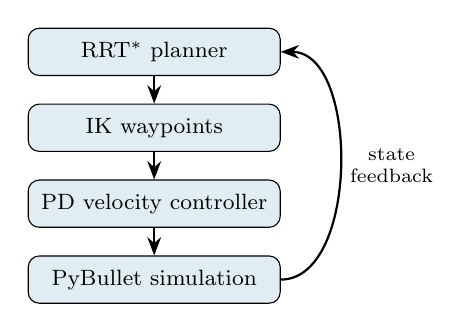
\begin{tikzpicture}[
          node distance=0.35cm and 0.2cm,
          block/.style={rectangle, draw, rounded corners, fill=accent!15,
                        minimum width=3.2cm, minimum height=0.6cm,
                        align=center, font=\footnotesize},
          arrow/.style={-Stealth, thick},
        ]
        \node[block] (plan) {RRT$^*$ planner};
        \node[block, below=of plan] (ik)   {IK waypoints};
        \node[block, below=of ik]   (pd)   {PD velocity controller};
        \node[block, below=of pd]   (sim)  {PyBullet simulation};
        \draw[arrow] (plan) -- (ik);
        \draw[arrow] (ik) -- (pd);
        \draw[arrow] (pd) -- (sim);
        \draw[arrow] (sim.east) .. controls +(1.0,0) and +(1.0,0) .. (plan.east)
              node[midway, right, font=\scriptsize, align=center] {state\\ feedback};
      \end{tikzpicture}
      \vspace{0.5em}
      \scriptsize M1 block diagram
    \end{column}
  \end{columns}
\end{frame}

% ---------------------------------------------------------------- Slide 5
\begin{frame}{M1 \(\to\) M2 --- The Stress Test}
  \textbf{Now perturb the cube pose just before execution.}

  \vspace{0.5em}
  \begin{center}
    \small
    \begin{tabular}{lccccccc}
      \toprule
      XY perturb (m) & 0.00 & 0.02 & 0.04 & 0.06 & 0.08 & 0.10 & 0.12 \\
      \midrule
      Planner success & 1.00 & 0.46 & 0.45 & 0.29 & 0.19 & 0.25 & 0.22 \\
      \bottomrule
    \end{tabular}
  \end{center}

  \vspace{0.5em}
  \begin{itemize}
    \item \textbf{Why it breaks:} IK was solved from the
          \emph{pre-perturbation} cube pose. The pre-computed joint
          waypoints no longer point at the real cube.
    \item The PD controller faithfully tracks \emph{stale} targets.
    \item The planner has no run-time perception feedback.
  \end{itemize}

  \vspace{0.5em}
  \alert{This is the gap residual RL fills.}
\end{frame}

% ---------------------------------------------------------------- Slide 6
\begin{frame}{M2 Architecture --- Residual on PD + IK}
  \centering
  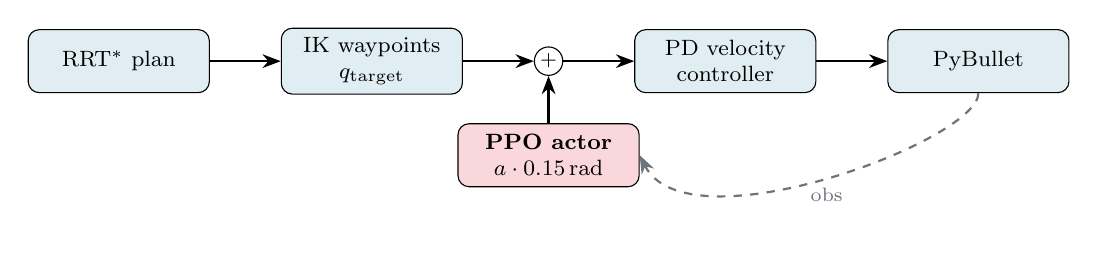
\begin{tikzpicture}[
      node distance=0.5cm and 0.9cm,
      block/.style={rectangle, draw, rounded corners, fill=accent!15,
                    minimum width=2.3cm, minimum height=0.8cm,
                    align=center, font=\footnotesize},
      rlblock/.style={rectangle, draw, rounded corners, fill=accent2!20,
                      minimum width=2.3cm, minimum height=0.8cm,
                      align=center, font=\footnotesize},
      sum/.style={circle, draw, inner sep=0.8pt, font=\scriptsize, fill=white},
      arrow/.style={-Stealth, thick},
    ]
    \node[block] (plan) {RRT$^*$ plan};
    \node[block, right=of plan] (ik) {IK waypoints \\ $q_{\text{target}}$};
    \node[sum, right=of ik] (sum) {$+$};
    \node[block, right=of sum] (pd) {PD velocity \\ controller};
    \node[block, right=of pd] (sim) {PyBullet};
    \node[rlblock, below=of sum, yshift=-0.1cm] (rl)
      {\textbf{PPO actor} \\ $a \cdot 0.15$\,rad};

    \draw[arrow] (plan) -- (ik);
    \draw[arrow] (ik) -- (sum);
    \draw[arrow] (sum) -- (pd);
    \draw[arrow] (pd) -- (sim);
    \draw[arrow] (rl) -- (sum);
    \draw[arrow, dashed, mutedgray] (sim.south) .. controls +(0,-0.6) and +(0.6,-1.2) .. (rl.east)
          node[midway, below, font=\scriptsize, align=center] {obs};
  \end{tikzpicture}

  \vspace{0.5em}
  \textbf{Key design choices:}
  \begin{itemize}
    \item \textbf{Position residual} (not velocity) --- stable learning, PD does tracking.
    \item \textbf{Bounded} --- $\lVert a \rVert_\infty \cdot 0.15$\,rad per joint.
    \item \textbf{Phase-gated} --- residual active only in \textsc{pre\_grasp}
          and \textsc{grasp\_descend}; disabled in \textsc{lift}.
  \end{itemize}
\end{frame}

% ---------------------------------------------------------------- Slide 7
\begin{frame}{Observation, Action, Reward}
  \small
  \begin{columns}[T]
    \begin{column}{0.52\textwidth}
      \textbf{Observation (41-d, fixed-scale normalized)}
      \begin{itemize}\setlength\itemsep{0.1em}
        \item joint $q$ (7) and $\dot q$ (7)
        \item EE pose: position (3) + Euler (3)
        \item cube pose: position (3) + Euler (3)
        \item EE\,$\to$\,cube vector (3)
        \item PD nominal $\dot q_{\text{PD}}$ (7)
        \item phase indicator (1)
        \item perturbation offset (3)
        \item waypoint progress (1)
      \end{itemize}

      \textbf{Action (7-d)}
      \begin{itemize}\setlength\itemsep{0.1em}
        \item clipped $[-1, 1]$, scaled by \texttt{RESIDUAL\_MAX\_POS}\,=\,0.15\,rad
      \end{itemize}
    \end{column}
    \begin{column}{0.48\textwidth}
      \textbf{Reward (per step, 11 terms)}
      \[
        r = r_{\text{shape}} + r_{\text{grasp}} + r_{\text{lift}}
            - r_{\text{fail}} - \lambda_r\lVert r^{\text{res}}\rVert_1
            - \lambda_s\lVert r^{\text{res}}\rVert_2^2 - c_\tau
      \]
      \begin{itemize}\setlength\itemsep{0.1em}
        \item $r_{\text{shape}}$: $\Delta$-distance approach +
              one-shot milestones (0.08/0.05/0.03\,m) + geom shaping at
              attempt + attempt bonus
        \item $\lambda_r, \lambda_s$: $\ell_1$ / $\ell_2^2$ on the
              \emph{residual vector} (not $\Delta a$)
        \item $r_{\text{grasp}}$: one-shot on geometric grasp gate
        \item $r_{\text{lift}}$: terminal on successful lift
        \item $r_{\text{fail}}$: terminal on cube fall; $c_\tau$: small
              per-step time cost, pre-attach only
      \end{itemize}
    \end{column}
  \end{columns}
\end{frame}

% ---------------------------------------------------------------- Slide 8
\begin{frame}{Training Setup}
  \small
  \begin{columns}[T]
    \begin{column}{0.50\textwidth}
      \textbf{Framework}
      \begin{itemize}
        \item TorchRL PPO, headless PyBullet
        \item 8 parallel workers, 1\,M frames total
        \item Actor: $2{\times}256$ Tanh + learnable log-std;
              critic: $512{\to}256$ Tanh
      \end{itemize}

      \textbf{Key hyperparameters}
      \begin{itemize}
        \item LR $5\!\times\!10^{-5}$ (linear decay $\to 0$), clip 0.2
        \item $\gamma{=}0.99$, GAE $\lambda{=}0.95$, 4 epochs, batch 8192
        \item Entropy $0.015 \to 0.005$ (linear); grad-clip 0.5; critic coef 0.5
        \item Target-KL early stop at 0.05 (100k-frame warmup)
      \end{itemize}
    \end{column}
    \begin{column}{0.50\textwidth}
      \textbf{Infrastructure}
      \begin{itemize}
        \item TensorBoard logging of reward, KL, entropy
        \item Composite smoothed best-model selection
              (grasp rate $+$ reward, nan-safe)
        \item Warm-start from proximity-shaped pre-training
              (hybrid only; rl\_only needs random init)
        \item CLI: \texttt{--mode}, \texttt{--seed}, \texttt{--workers}, \texttt{--resume}
      \end{itemize}
    \end{column}
  \end{columns}

  \vspace{0.5em}
  \textbf{Baselines evaluated alongside hybrid:}
  \texttt{planner\_only} (residual zeroed) and
  \texttt{rl\_only} (policy commands full velocity, no PD backbone).
\end{frame}

% ---------------------------------------------------------------- Slide 9
\begin{frame}{Iteration Journey --- What Went Wrong, What We Fixed}
  \small
  \textbf{Six days of aggressive iteration (Apr 13--19) uncovered five real bugs:}

  \vspace{0.3em}
  \begin{enumerate}
    \item \textbf{Velocity} residual $\to$ \textbf{position} residual.
          Velocity-additive residual was destabilising the PD loop; the position
          formulation let PD do the tracking.
    \item \textbf{Reward hacking.} Proximity shaping dominated; agent hovered
          near the cube without attempting a grasp. Capped proximity +
          emphasised terminal bonuses.
    \item \textbf{Reward attractor was at the nominal cube pose.} The policy
          was incentivised to approach the wrong point. Re-centred it on the
          post-perturbation cube each reset.
    \item \textbf{Grasp gate accepted bad contacts.}
          Added below-top, finger-bracket, and opposite-face perpendicularity
          checks plus a fingertip-offset correction.
    \item \textbf{Planner@nominal anomaly.} Classical planner dropped below
          100\% at zero perturbation. Root cause: joint-waypoint tolerance
          compounded to $\sim$1\,cm Cartesian error. Fix: Cartesian settle loop
          before closing the gripper.
  \end{enumerate}
\end{frame}

% ==================================================================
% SECTION: DEMOS / RESULTS
% ==================================================================

% ---------------------------------------------------------------- Slide 10
\begin{frame}{Evaluation Protocol}
  \textbf{2100 episodes total:} 3 methods $\times$ 7 perturbation levels $\times$ 100 episodes.

  \vspace{0.5em}
  \begin{itemize}
    \item \textbf{Methods:} \texttt{planner\_only}, \texttt{hybrid} (PD + residual), \texttt{rl\_only}
    \item \textbf{Perturbation levels:} XY $\in \{0.00, 0.02, 0.04, 0.06, 0.08, 0.10, 0.12\}$\,m
          (with Z and yaw scaled proportionally)
    \item \textbf{Metrics:}
          \begin{itemize}
            \item success rate (Wilson 95\% CI)
            \item mean reward, mean residual magnitude (rad)
            \item mean EE--cube distance at grasp attempt
            \item episode length, phase distribution at termination
          \end{itemize}
    \item \textbf{Actions:} stochastic (match training distribution)
    \item \textbf{Single seed per policy} --- noted limitation, multi-seed deferred to M3
  \end{itemize}
\end{frame}

% ---------------------------------------------------------------- Slide 11
\begin{frame}{Headline Result --- Success vs.\ Perturbation}
  \begin{columns}[T]
    \begin{column}{0.62\textwidth}
      \centering
      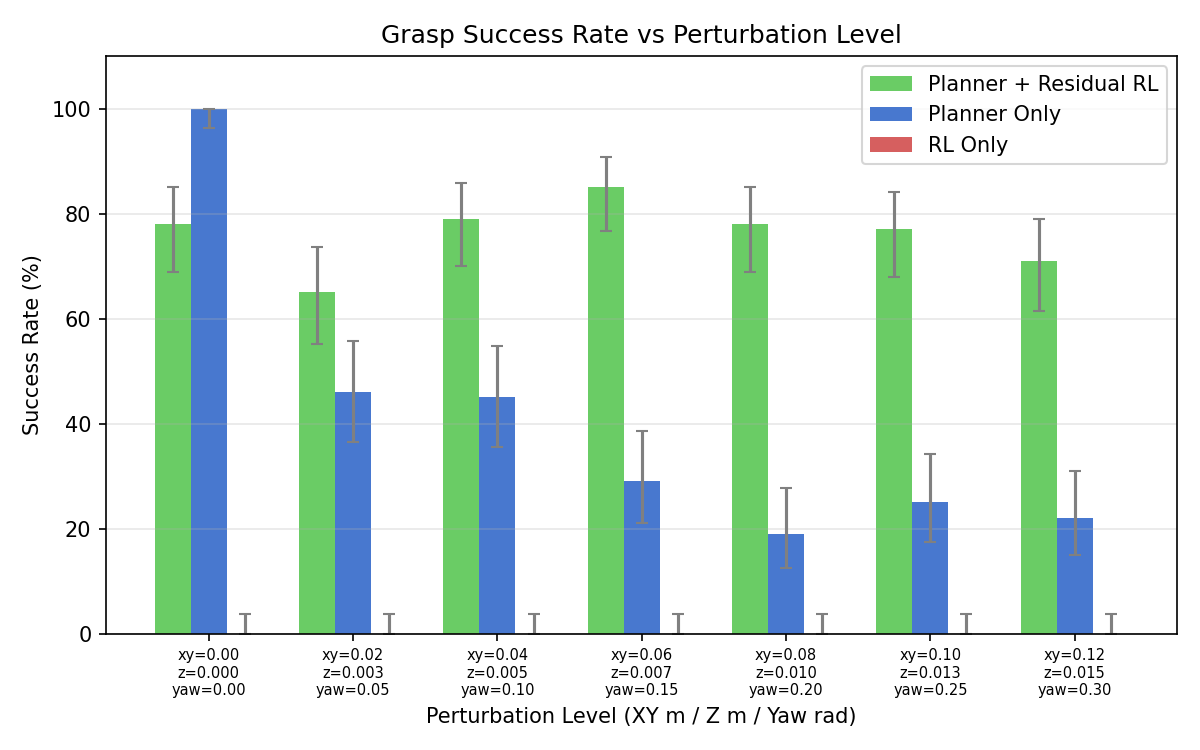
\includegraphics[width=\linewidth]{success_rate_vs_perturbation.png}
    \end{column}
    \begin{column}{0.38\textwidth}
      \footnotesize
      \textbf{Planner} (blue): 1.00 $\to$ 0.22 \\
      cliff at 2\,cm perturbation.

      \vspace{0.5em}
      \textbf{Hybrid} (orange): \alert{0.65--0.85} \\
      flat across all 7 levels.

      \vspace{0.5em}
      \textbf{RL-only} (grey): 0.00 \\
      every level.

      \vspace{1em}
      \textbf{34--59 pp} gap over the planner at XY\,$\geq$\,0.04\,m (peak 59 pp at 8\,cm).

      \vspace{0.5em}
      \textcolor{mutedgray}{Hybrid at nominal (0.78) $<$ planner
      at nominal (1.00) --- discussed later.}
    \end{column}
  \end{columns}
\end{frame}

% ---------------------------------------------------------------- Slide 12
\begin{frame}{The Policy is Actively Correcting}
  \begin{columns}[T]
    \begin{column}{0.58\textwidth}
      \centering
      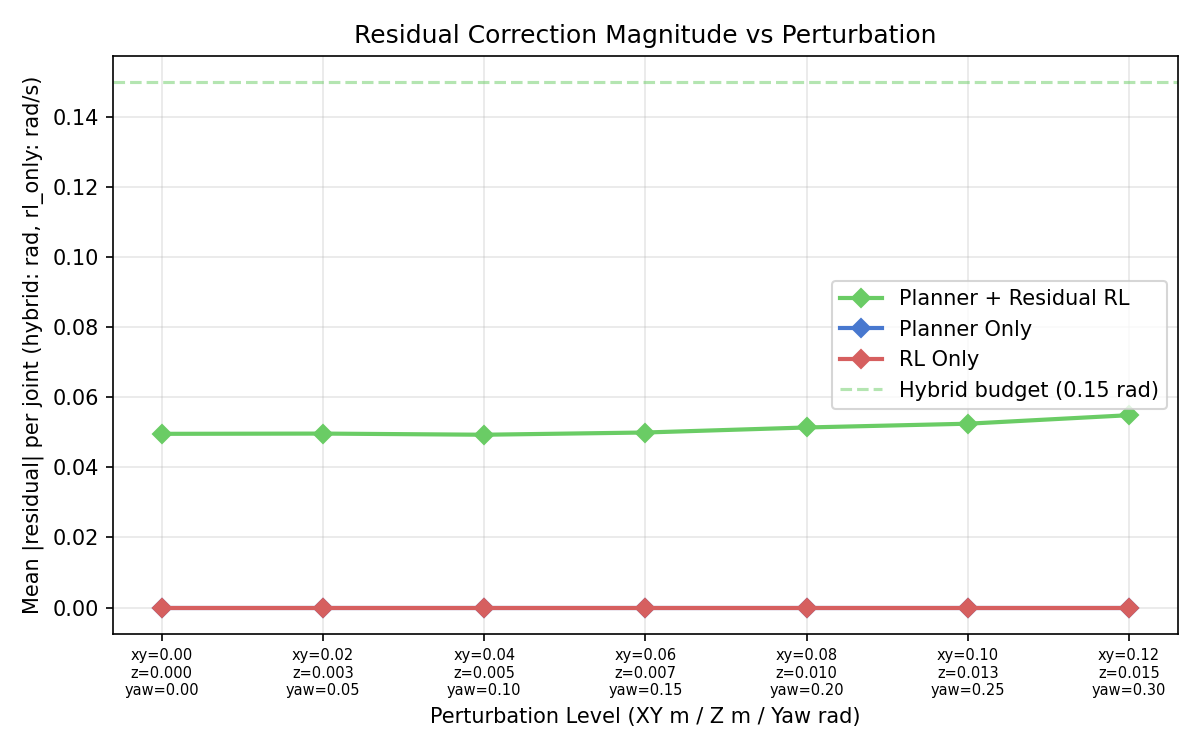
\includegraphics[width=\linewidth]{residual_magnitude.png}
    \end{column}
    \begin{column}{0.42\textwidth}
      \footnotesize
      \textbf{Residual magnitude (hybrid)} \\
      Mean $\approx$ \alert{0.050--0.055 rad} \\
      (33--37\% of the 0.15\,rad budget).

      \vspace{1em}
      \textbf{EE--cube distance at grasp:}
      \begin{itemize}
        \item Hybrid: \alert{0.018--0.026\,m} across all levels
        \item Planner: 0.020\,m nominal $\to$ 0.056\,m at XY\,=\,0.12\,m
      \end{itemize}

      \vspace{0.5em}
      \alert{The residual cancels the planner's drift.}
      Evidence the correction is load-bearing, not cosmetic.
    \end{column}
  \end{columns}
\end{frame}

% ---------------------------------------------------------------- Slide 13
\begin{frame}{Ablation --- \texttt{rl\_only} Fails Everywhere}
  \begin{columns}[T]
    \begin{column}{0.55\textwidth}
      \centering
      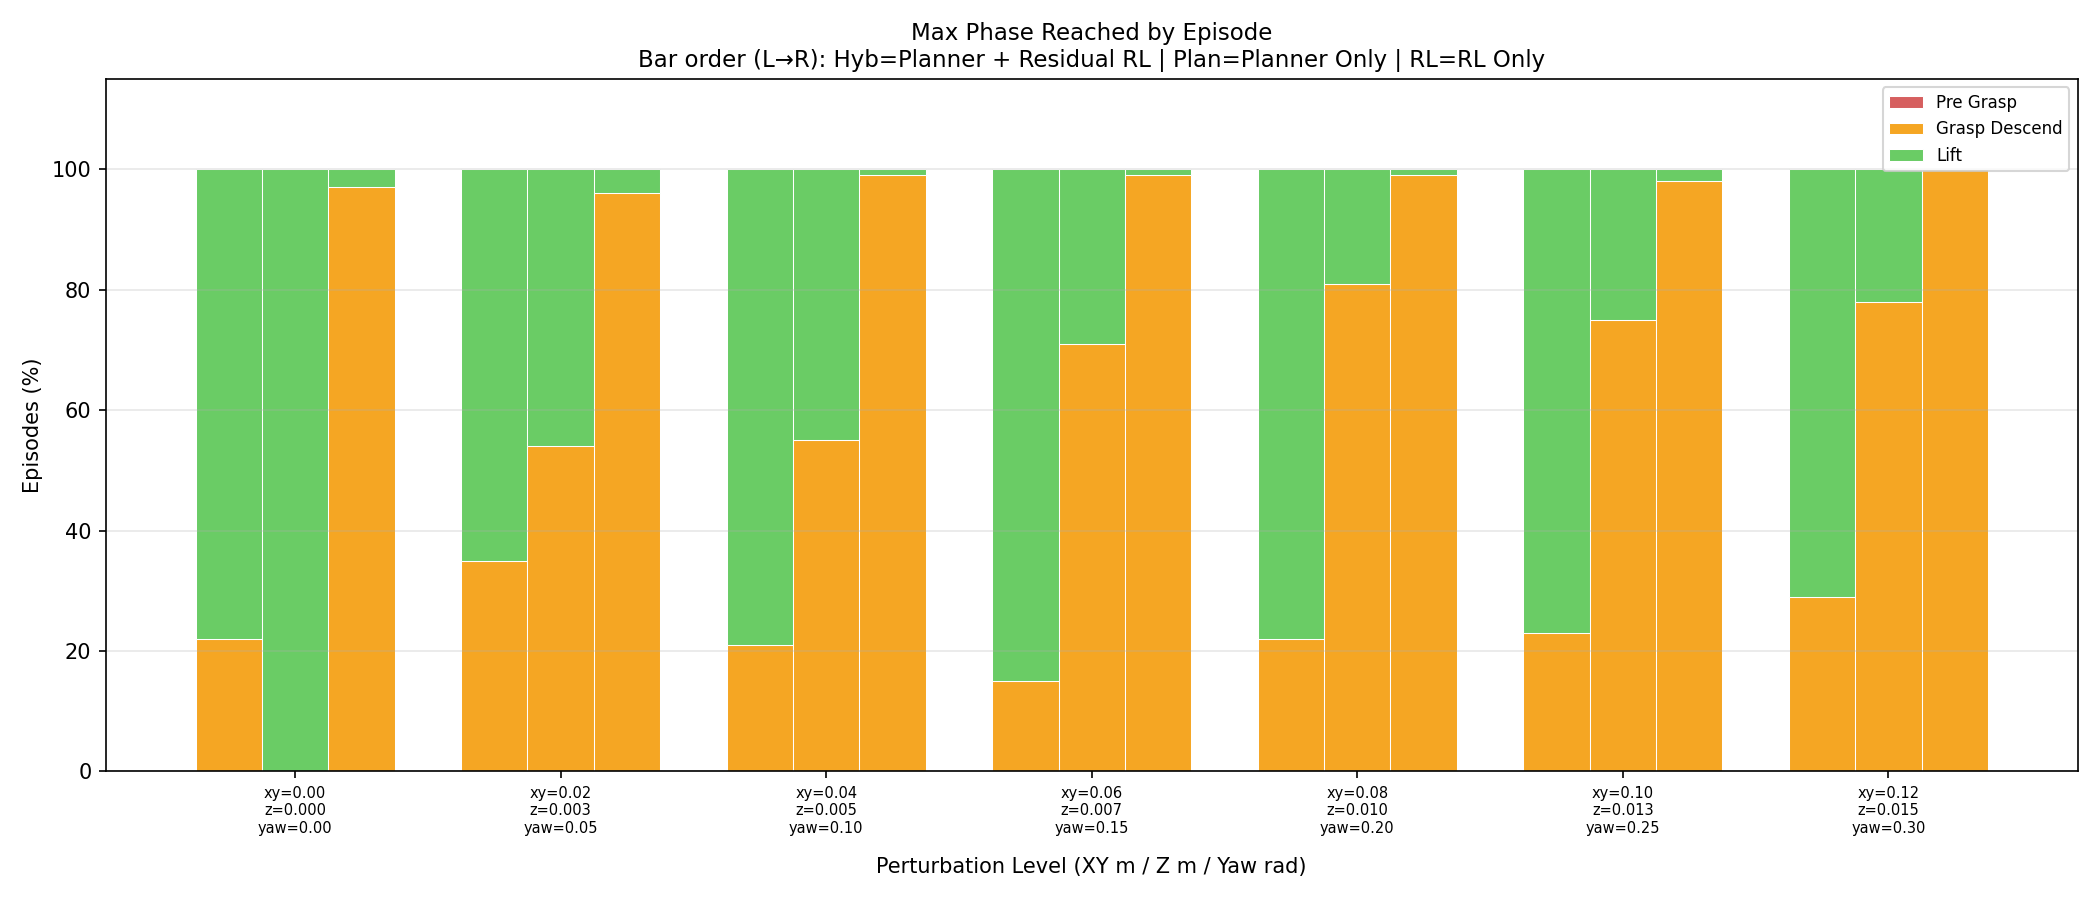
\includegraphics[width=\linewidth]{phase_breakdown.png}
    \end{column}
    \begin{column}{0.45\textwidth}
      \footnotesize
      \textbf{\texttt{rl\_only}} (no PD backbone):
      \begin{itemize}
        \item Stuck in \textsc{grasp\_descend} 96--100\% of episodes per level
        \item 0\% lifts at every perturbation level
        \item EE--cube distance flat at \alert{0.10\,m}
              --- no cube tracking learned
      \end{itemize}

      \vspace{0.8em}
      \textbf{Takeaway:} removing the PD+IK scaffold wastes the budget
      re-learning behaviour the classical stack already provides.
      \alert{The backbone is load-bearing.}
    \end{column}
  \end{columns}
\end{frame}

% ---------------------------------------------------------------- Slide 14
\begin{frame}{Demo Reel --- Planner Fails, Hybrid Recovers}
  \small
  Same perturbation (XY\,=\,4\,cm, Z\,=\,5\,mm, yaw\,=\,0.10\,rad).
  Different controllers. Played live from the ZIP.

  \vspace{0.3em}
  \begin{columns}[T]
    \begin{column}{0.48\textwidth}
      \centering
      % \includegraphics[width=\linewidth]{demo_thumb_planner_004.png}
      \fbox{\parbox[c][4.0cm][c]{\linewidth}{\centering \textbf{Planner Only @ perturbed}\\[0.4em]\textit{Planner Only Perturb xy0.04 z0.005 yaw0.10.mp4}\\[0.4em] gripper closes on empty space}}
      \vspace{0.2em}\\
      \scriptsize \textbf{Planner} --- stale IK target, grasp misses.
    \end{column}
    \begin{column}{0.48\textwidth}
      \centering
      % \includegraphics[width=\linewidth]{demo_thumb_hybrid_004.png}
      \fbox{\parbox[c][4.0cm][c]{\linewidth}{\centering \textbf{Hybrid @ perturbed}\\[0.4em]\textit{Hybrid Perturb xy0.04 z0.005 yaw0.10.mp4}\\[0.4em] residual bar grows on descend, grasp lands}}
      \vspace{0.2em}\\
      \scriptsize \textbf{Hybrid} --- residual steers the EE onto the real cube.
    \end{column}
  \end{columns}

  \vspace{0.3em}
  \scriptsize\textit{Overlay: residual bar shows commanded position offset
  magnitude (rad) relative to the 0.15\,rad budget.}
\end{frame}

% ---------------------------------------------------------------- Slide 15
\begin{frame}{Demo Reel --- Nominal Baseline vs.\ \texttt{rl\_only} Ablation}
  \small
  \begin{columns}[T]
    \begin{column}{0.48\textwidth}
      \centering
      % \includegraphics[width=\linewidth]{demo_thumb_planner_nominal.png}
      \fbox{\parbox[c][4.0cm][c]{\linewidth}{\centering \textbf{Planner Only @ nominal}\\[0.4em]\textit{Planner Only Perturb xy0.0 z0.0 yaw0.0.mp4}\\[0.4em] clean 11-phase pick-and-place}}
      \vspace{0.2em}\\
      \scriptsize \textbf{Planner @ nominal} --- the baseline that was brittle under perturbation.
    \end{column}
    \begin{column}{0.48\textwidth}
      \centering
      % \includegraphics[width=\linewidth]{demo_thumb_rlonly_004.png}
      \fbox{\parbox[c][4.0cm][c]{\linewidth}{\centering \textbf{RL Only @ perturbed}\\[0.4em]\textit{RL Only Perturb xy0.04 z0.005 yaw0.10.mp4}\\[0.4em] EE never reaches the cube}}
      \vspace{0.2em}\\
      \scriptsize \textbf{RL-only} --- learned joint scaffold, not cube tracking.
    \end{column}
  \end{columns}

  \vspace{0.3em}
  \scriptsize\textit{Removing the PD+IK backbone forces the policy to
  re-learn what the classical stack already provides --- and it fails
  to close the Cartesian loop on the real cube.}
\end{frame}

% ---------------------------------------------------------------- Slide 16
\begin{frame}{Discussion \& Limitations}
  \small
  \begin{itemize}
    \item \textbf{Hybrid @ nominal (0.78) $<$ planner @ nominal (1.00).}
          The residual is always on; at zero perturbation its noise
          occasionally drives the EE off a correct plan. A
          confidence-gated residual (only active when the cube
          disagrees with the plan) is an obvious next step.
    \item \textbf{Single seed per policy.} Multi-seed evaluation is
          deferred to M3 to tighten the confidence intervals.
    \item \textbf{Geometric grasp check is a heuristic.} Below-top +
          bracket + opposite-face perpendicularity catches the obvious
          failure modes but does not test real force closure.
          A learned grasp gate is an M3 candidate.
    \item \textbf{Perturbation is XY-dominant.} Z and yaw are scaled
          proportionally; richer orientation and clutter perturbations
          are M3 work.
  \end{itemize}
\end{frame}

% ==================================================================
% SECTION: FUTURE WORK / REMAINING / CONTRIBUTIONS
% ==================================================================

% ---------------------------------------------------------------- Slide 17
\begin{frame}{Future Work, Remaining, Contributions}
  \small
  \begin{columns}[T]
    \begin{column}{0.33\textwidth}
      \textbf{\textcolor{accent3}{M3 plan}}
      \begin{itemize}
        \item Curriculum over perturbation magnitude
        \item Richer perturbation: full orientation, clutter, distractors
        \item Multi-seed, multi-run aggregation
        \item Refactor towards sim-to-real (domain randomisation, delayed obs)
      \end{itemize}
    \end{column}
    \begin{column}{0.33\textwidth}
      \textbf{\textcolor{accent2}{Stretch}}
      \begin{itemize}
        \item Learned grasp gate (replace heuristic)
        \item Confidence-gated residual (address nominal regression)
        \item Real-robot transfer (Panda, table-top pick-place)
      \end{itemize}
    \end{column}
    \begin{column}{0.33\textwidth}
      \textbf{Remaining for PM2}
      \begin{itemize}
        \item Record the 10-min Zoom talk
        \item Package README + demo videos + code ZIP
      \end{itemize}
      \vspace{0.5em}
      \textbf{Contributions}
      \begin{itemize}
        \item \textbf{[Member A]:} [role]
        \item \textbf{[Member B]:} [role]
      \end{itemize}
    \end{column}
  \end{columns}
\end{frame}

% ---------------------------------------------------------------- Slide 18
\begin{frame}[standout]
  Thank you.

  \vspace{1em}
  \normalsize
  Questions?

  \vspace{2em}
  \scriptsize
  Repo: \texttt{github.com/john-2424/cs558rob} \\
  Contact: \texttt{krishnarajule3@gmail.com}
\end{frame}

% ==================================================================
% APPENDIX (backup slides for Q\&A)
% ==================================================================
\appendix

\begin{frame}{Appendix --- Mean Reward vs.\ Perturbation}
  \centering
  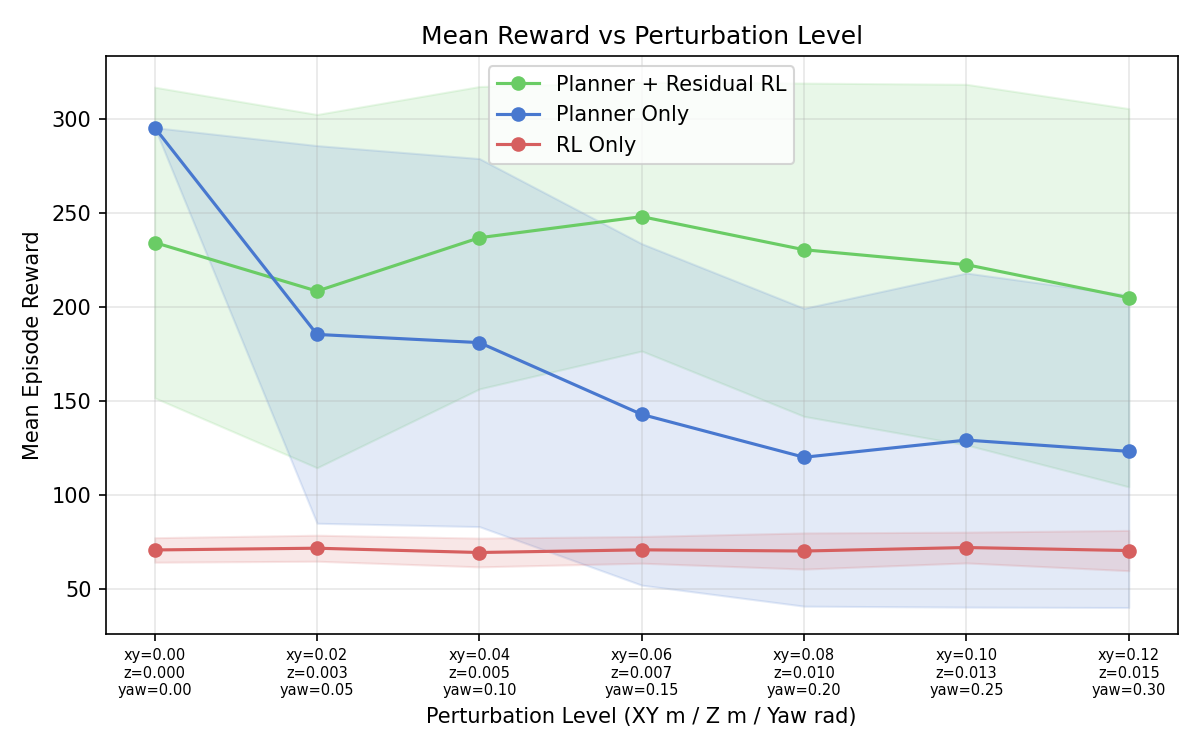
\includegraphics[width=0.75\linewidth]{mean_reward_vs_perturbation.png}
\end{frame}

\begin{frame}{Appendix --- Episode Length vs.\ Perturbation}
  \centering
  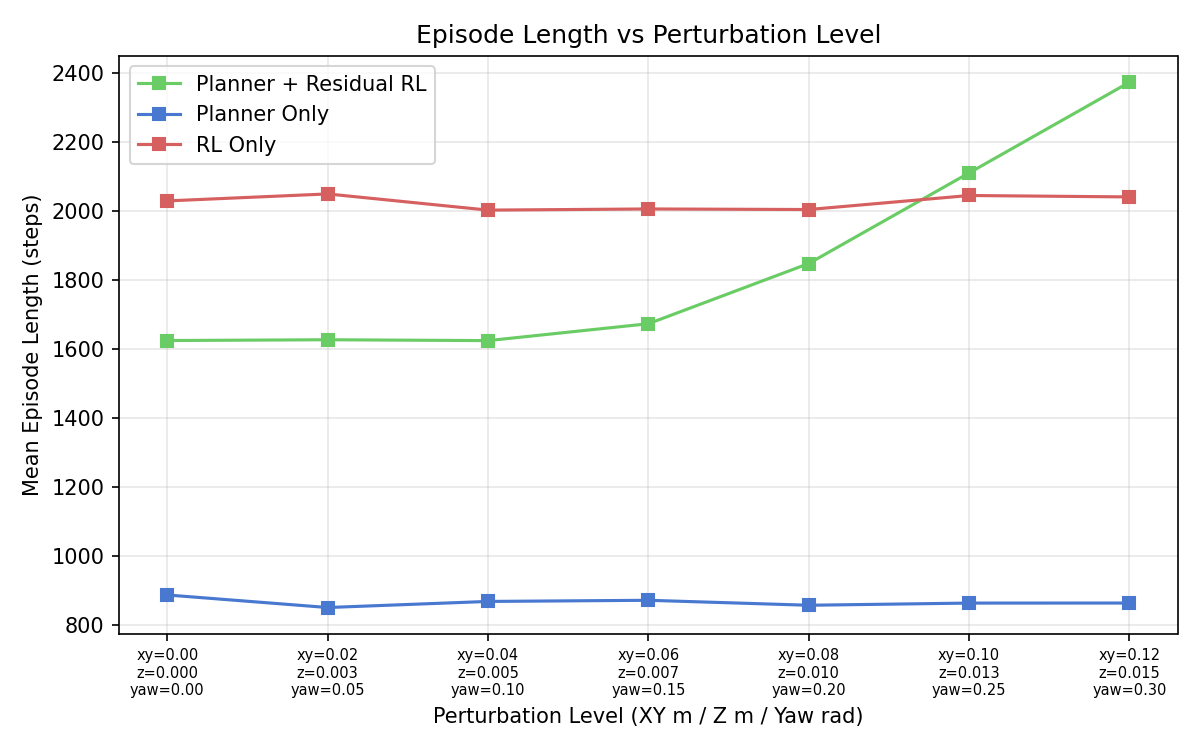
\includegraphics[width=0.75\linewidth]{episode_length_vs_perturbation.png}
\end{frame}

\begin{frame}{Appendix --- Diagnostic Metrics}
  \centering
  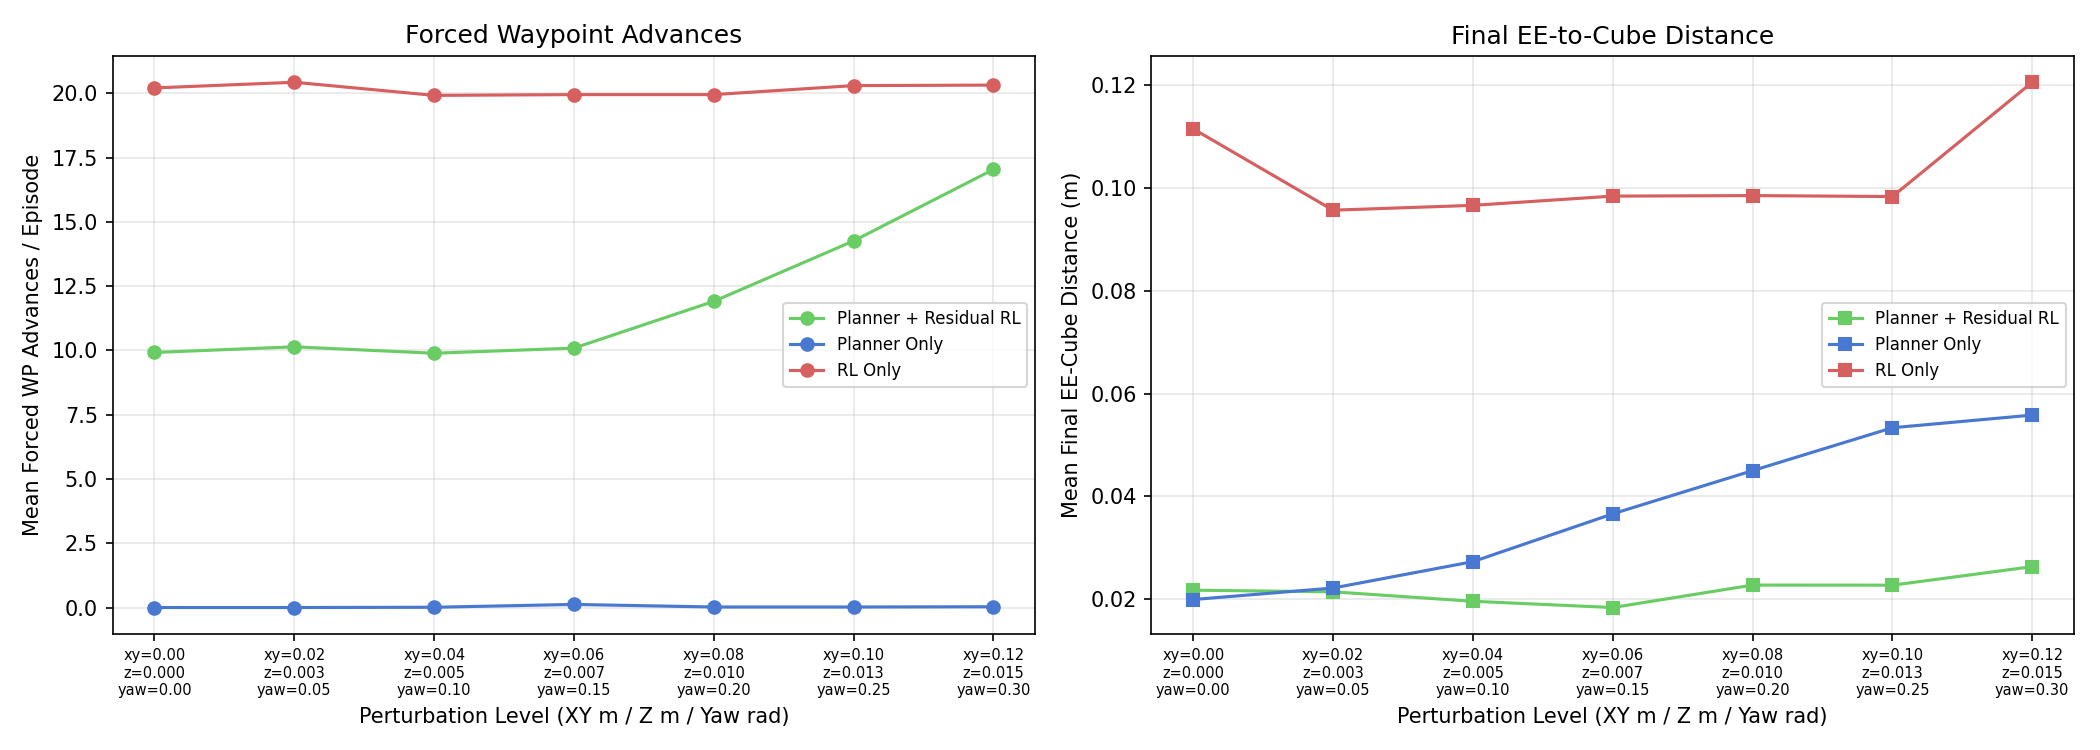
\includegraphics[width=0.75\linewidth]{diagnostic_metrics.png}
\end{frame}

\begin{frame}{Appendix --- Summary Table}
  \centering
  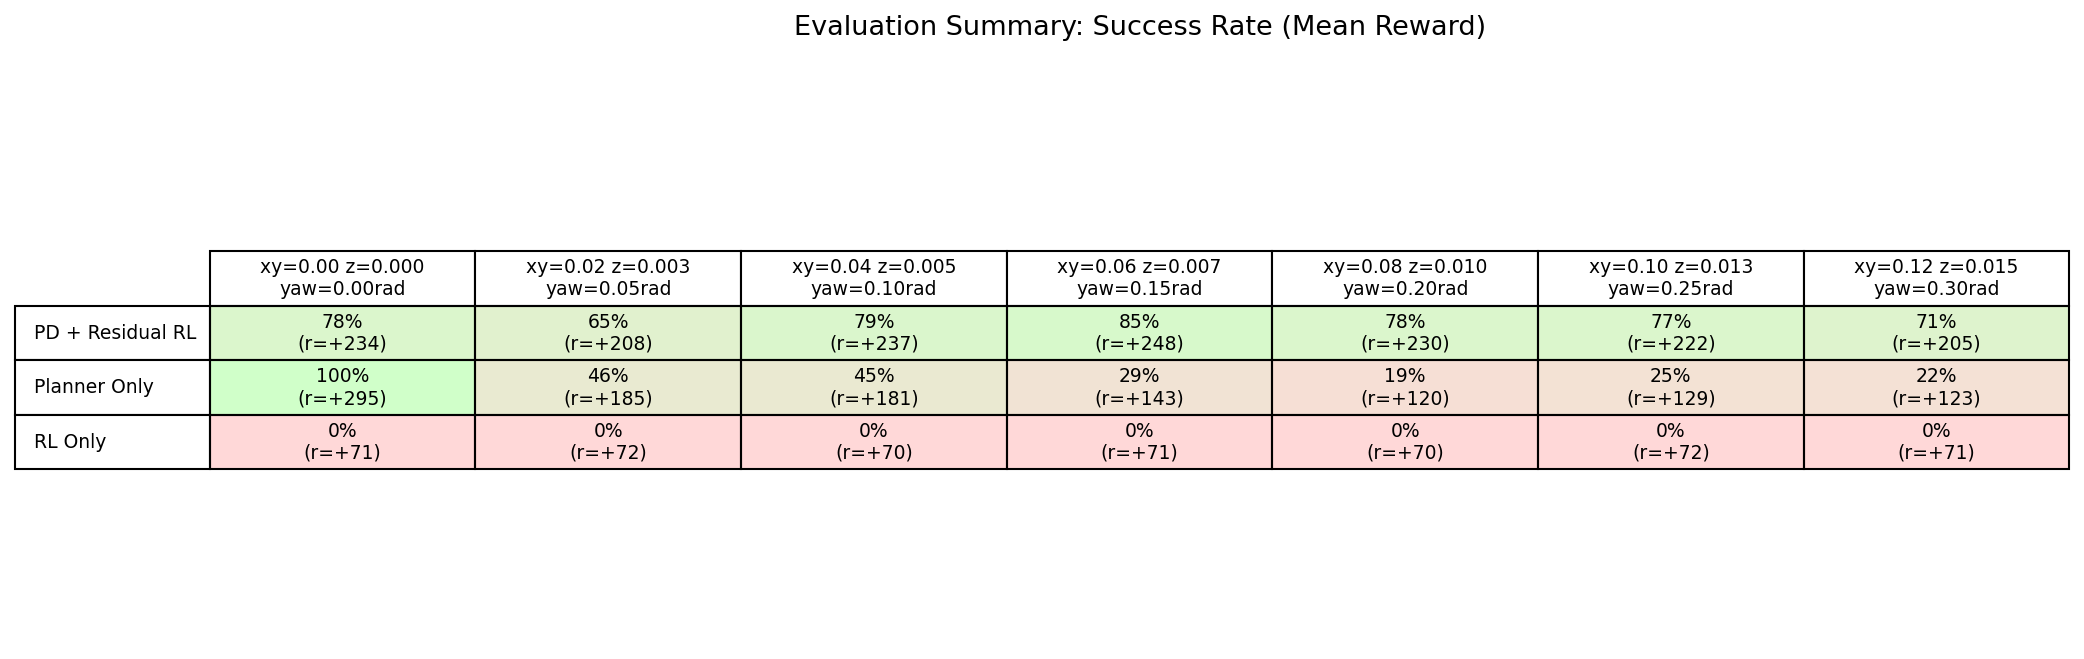
\includegraphics[width=0.85\linewidth]{summary_table.png}
\end{frame}

\begin{frame}{Appendix --- Grasp Analysis}
  \centering
  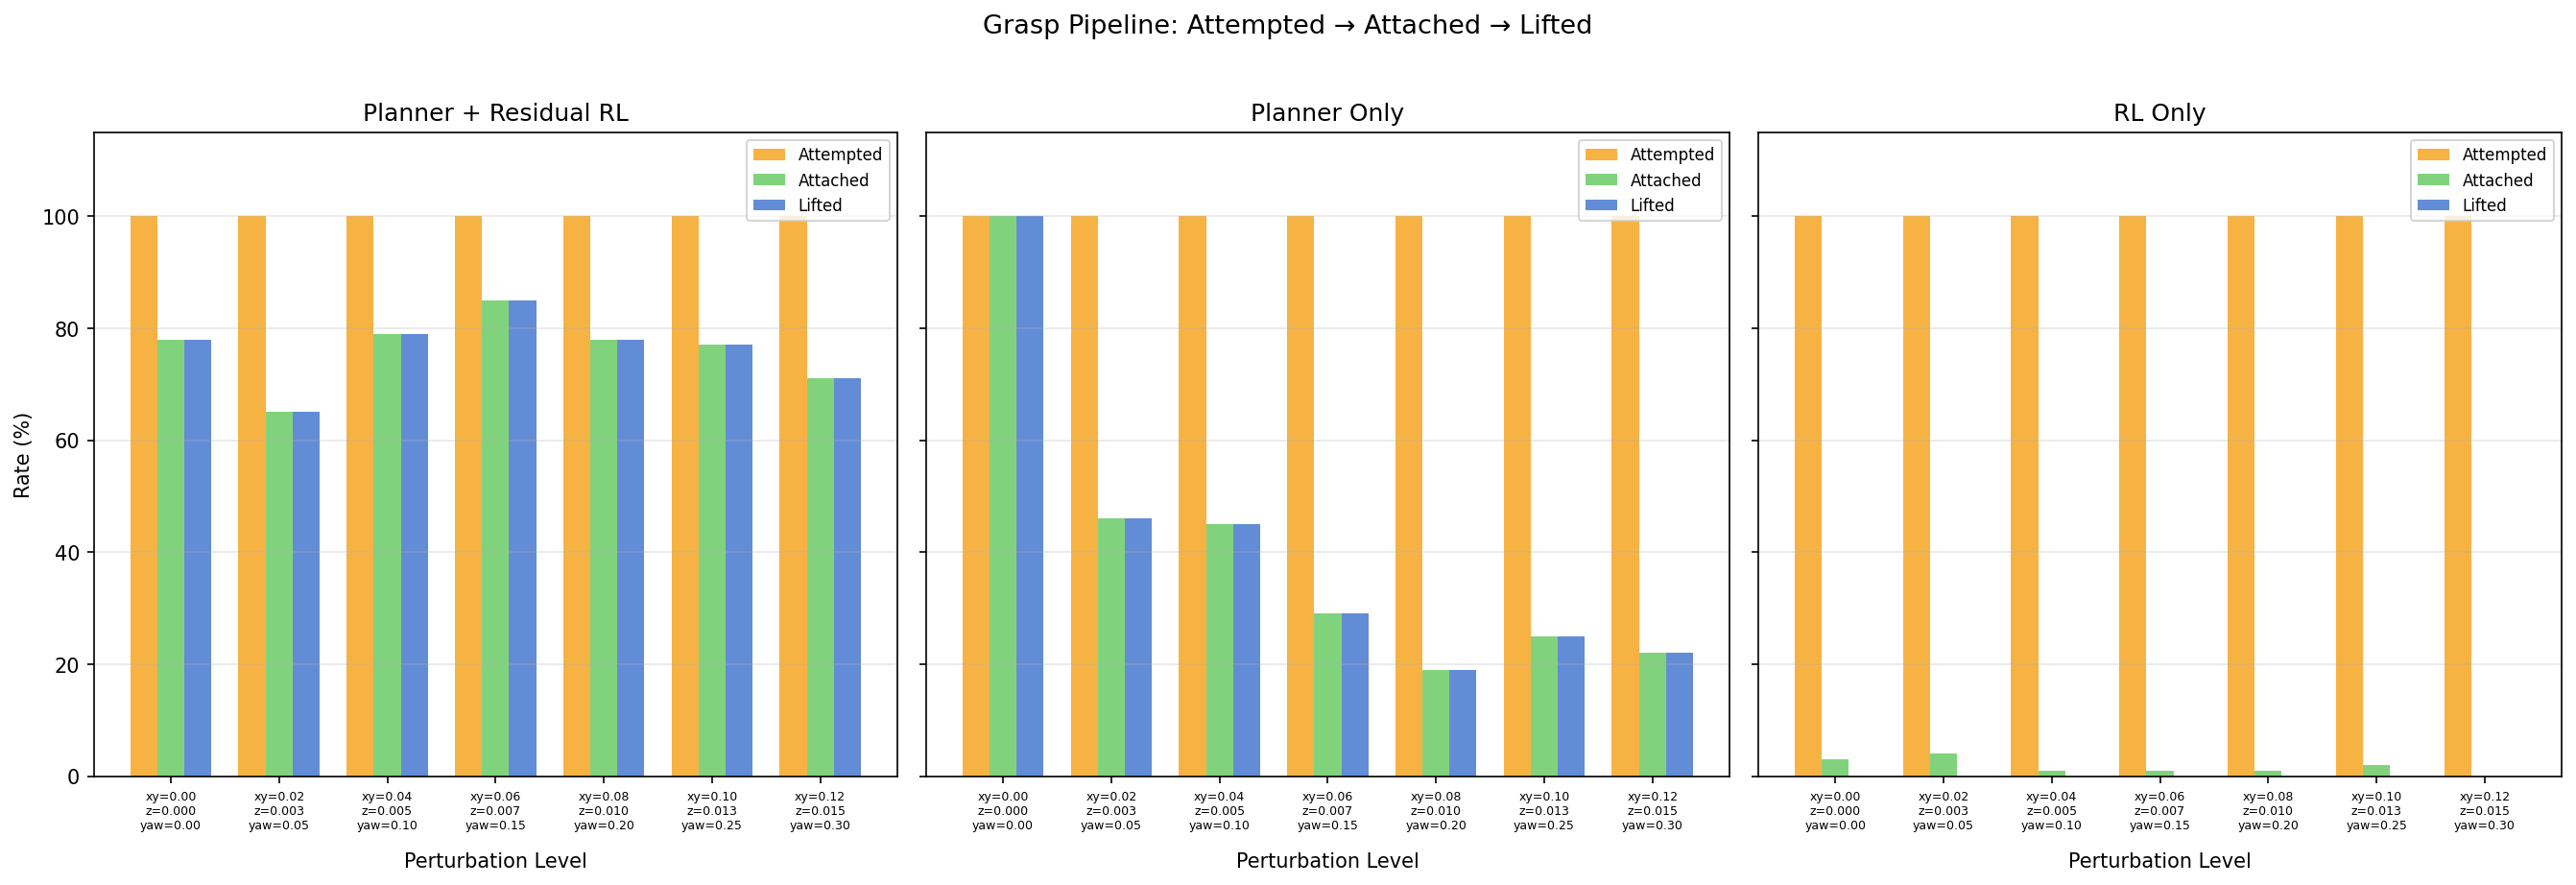
\includegraphics[width=0.75\linewidth]{grasp_analysis.png}
\end{frame}

\end{document}
